\documentclass{article}
\usepackage{amsmath}
\usepackage{amssymb}
\usepackage{graphicx}
\usepackage{hyperref}
\usepackage[version=4]{mhchem}


\begin{document}
\section*{Problem}
(AMC) Let line \(A C\) be perpendicular to line \(C E\). Connect \(A\) to the midpoint \(D\) of \(C E\), and connect \(E\) to the midpoint \(B\) of \(A C\). If \(A D\) and \(E B\) intersect in point \(F\), and \(B C=C D=15\) inches, find the area of triangle \(D F E\) in square inches.

\section*{Solution}
(C).\\
We draw the height from \(A\) to the base \(B C\) as shown in the figure to the right.\\
Triangle \(A D C\) is a \(30^{\circ}-60^{\circ}-90^{\circ}\) right triangle, and so the ratio of the sides is \(1: \sqrt{3}: 2\). It follows that \(A D=\) \(16 / 2=8\) and \(C D=8 \sqrt{3}\).\\
Triangle \(A D B\) is a \(45^{\circ}-45^{\circ}-90^{\circ}\) right triangle, and so\\
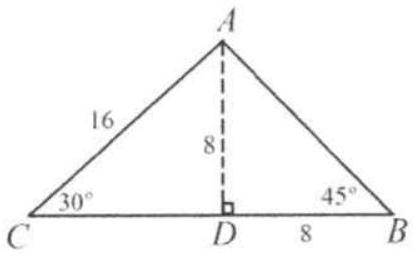
\includegraphics[width=\textwidth]{images/092.jpg} the ratio of the sides is \(1: \quad 1: \sqrt{2}\). Thus, \(D B=8\).\\
The answer is \(8+8 \sqrt{3}\).

\end{document}
